%Chapter 4

\renewcommand{\thechapter}{4}


\chapter{Absorption imaging in the presence of strong recoil induced detuning}


\section{On-resonant atom-light interaction}

\section{Absorption imaging}
Absorption imaging measures the shadow cast by an atomic ensemble in an illuminating probe laser beam with angular frequency $\omega_{\rm{L}}$. This imaging technique relies on optical transitions between ground and excited atomic states. Such atomic transitions have an energy difference $\hbar\omega_0$, and a natural transition linewidth $\Gamma$. When interacting with a laser field an atom scatters photons from the laser field into the vacuum modes. In the two-level atom approximation, the rate of scattering is \cite{LCT}
\begin{equation}
\gamma_{\rm{sc}}= \frac{\Gamma}{2} \frac{\tilde{I}}{1+4\tilde{\delta}^2 +\tilde{I}},
\label{eq:scatrate}
\end{equation}
where $\tilde{I}=I/I_{\rm{sat}}$ is the laser intensity in units of the saturation intensity, and $\tilde{\delta}=\delta/\Gamma$ is the detuning $\delta=\omega_{\rm{L}}-\omega_0$ in units of the natural linewidth. 
\par An absorption image is obtained by shining an on- or near-resonant probe beam ($\tilde{\delta}\ll1$) onto the atomic cloud. Some of the light is scattered by the atoms, and the unscattered light, $\tilde{I}_f(x,y)$, is imaged onto a camera, as depicted in Fig. \ref{fig:absorptionIntor}(a) (top). The probe light is reapplied with the atoms absent to calibrate the intensity $\tilde{I}_0(x,y)$ of light unaffected by the atoms (bottom).
\begin{figure}
	\subfigure[]{\includegraphics*[scale=0.5]{Chapter4 Figures/Picture1a}}
	\subfigure[]{\includegraphics*{Chapter4 Figures/Picture1c.pdf}}
	\subfigure[]{\includegraphics*[scale=0.55]{Chapter4 Figures/Picture1b}}
\caption{Absorption imaging. (a) Near resonant probe light illuminates the atoms, and the transmitted light (containing a shadow of the atoms) is imaged on the camera. A second image taken with no atoms provides a reference. (b)  The probe beam is partially absorbed as it traverses the cloud, and the intensity seen by atoms further along the imaging direction \ez{} is lowered.  (c) An atomic cloud illuminated by a probe light field absorbs photons from the probe and re-emits them in all directions. This process results in a net acceleration of the cloud in the direction of the probe light as well as diffusive spreading in the transverse directions.  }
\label{fig:absorptionIntor}
\end{figure}

The intensity $\tilde{I}_f(x,y)$ is related to the number of atoms the light encountered. Consider the light as it travels along the imaging axis \ez{} through a 3D atomic density profile $\rho(x,y,z)$. We focus on a single pixel of the camera: sensitive to a single column of atoms $\rho(z)$ giving  $\tilde{I}_0$ and $\tilde{I}_f$. Our task is to invert the problem and obtain a column density $n = \int \rho\left(z\right) \,\mathrm{d}z$ given $\tilde{I}_0$ and $\tilde{I}_f$. As the light travels through a column of atoms, each atom scatters light according to Eq. (\ref{eq:scatrate}). Therefore, the atoms further along the imaging axis $z$ experience a reduced optical intensity due to attenuation of the laser field by the other atoms (Fig. \ref{fig:absorptionIntor}(b)). The intensity change from scattering as a function of $z$ is
\begin{equation}
\frac{d\tilde{I}(z)}{dz}=-\hbar\omega_{\rm{L}}\rho(z)\gamma_{sc}(z)=-\rho(z)\sigma_0\frac{\tilde{I}(z)}{1+4\tilde{\delta}^2 +\tilde{I}},
\label{eq:dIdz}
\end{equation}
where $\sigma_0$ is the resonant scattering cross section. Integrating this equation yields a relation between the observed optical depth $OD=-\ln \left(I_f/I_0\right)$ and the atomic column density $n$ \cite{Reinaudi07} --- we call the column density deduced in this manner $\sigma_0 n^{\rm{(1)}}$:
\begin{equation}
\sigma_0 n^{\rm{(1)}} = \left(1+4\tilde{\delta}^2\right)OD+ \tilde{I}_0-\tilde{I}_f.
\label{eq2}
\end{equation}
When the probe intensity is much smaller than the saturation intensity, $\tilde{I}_0\ll1$, and the probe light is on resonance, $\tilde{\delta}=0$, the right hand side of Eq. (\ref{eq2}) reduces to the optical depth \cite{Reinaudi07}, giving the simple relationship $\sigma_0 n^{\rm{(0)}}=OD$. 
	\par Equations (\ref{eq:dIdz})-(\ref{eq2}) neglect the atomic recoil momentum and its effect on the laser detuning \cite{Konstantinidis12}. When an atom absorbs a photon from the laser light field it acquires a momentum kick $\hbar  k_{\rm{r}}$ in the direction of the light field. The associated recoil velocity is $v_{\rm{r}}=\hbar k_{\rm{r}}/m$, where $m$ is the atomic mass and $\hbar k_{\rm{r}}= h/\lambda$ is the recoil momentum from the laser with wavelength $\lambda$. Each re-emitted photon imparts a similar recoil momentum $\bf{\mathit{p}_e}$, but over many scattering events this momentum distribution averages to zero. Therefore the atom  will acquire an average velocity per photon $v_{\rm{r}}$ along \ez{}. The variance of $\bf{\mathit{p}_e}$, however, is not zero, allowing the atoms to acquire some momentum transverse to the laser field. While we ignore this correction, it results in the reduction of spatial resolution in the final image and its effect on the atomic cloud is pictured in Fig. \ref{fig:absorptionIntor}(c).


\section{Recoil-induced detuning}


\par The average atom velocity parallel the light field after scattering $N$ photons is $N v_{\rm{r}}$ and it is Doppler shifted  $\delta= k_{\rm{r}} N v_{\rm{r}}$ from resonance. For any probe intensity, there is an imaging time that we call the recoil time $t_{\rm{r}}$ after which  $\delta>\Gamma/2$ and, even if the probe beam is initially on resonance with the atomic transition, we cannot neglect the detuning's  effect on the scattering rate. Furthermore, this detuning varies both with imaging time $t$ and with distance along the propagation direction $z$ (Fig. \ref{fig:expos}(a)). Thus, the laser's spatially varying intensity profile in the atomic cloud also depends on time:
\begin{equation}
\frac{d\tilde{I}(t,z)}{dz}=-\sigma_0 \rho(t,z) \frac{\tilde{I}(t,z)}{1+4\tilde{\delta}(t,z)^2 +\tilde{I}(t,z)}. \label{eq3}
\end{equation}
Assuming that the atoms do not move significantly during the imaging time (we will remove this assumption shortly), the dimensionless detuning is
\begin{equation}
\tilde{\delta}(t,z)=\frac{ k_{\rm{r}} v_{\rm{r}}}{2\sigma_0 \rho(t,z)}\int_0^t \frac{d\tilde{I}(z,\tau)}{dz}\,\mathrm{d}\tau; \label{eq4}
\end{equation}
the relationship between the atomic density and the observed intensities is no longer straightforward.
\begin{figure}
	\subfigure[]{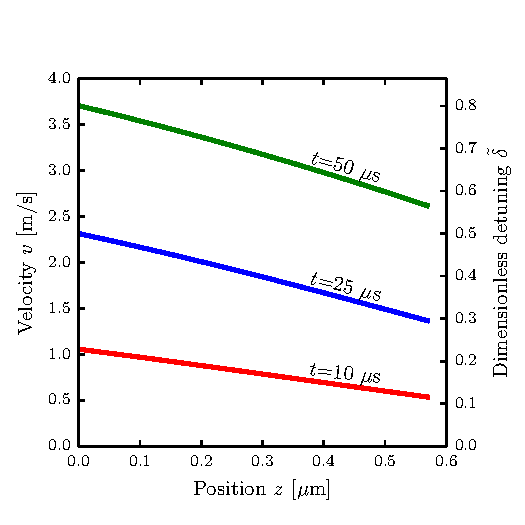
\includegraphics{Chapter4 Figures/figure1.pdf}}
	\subfigure[]{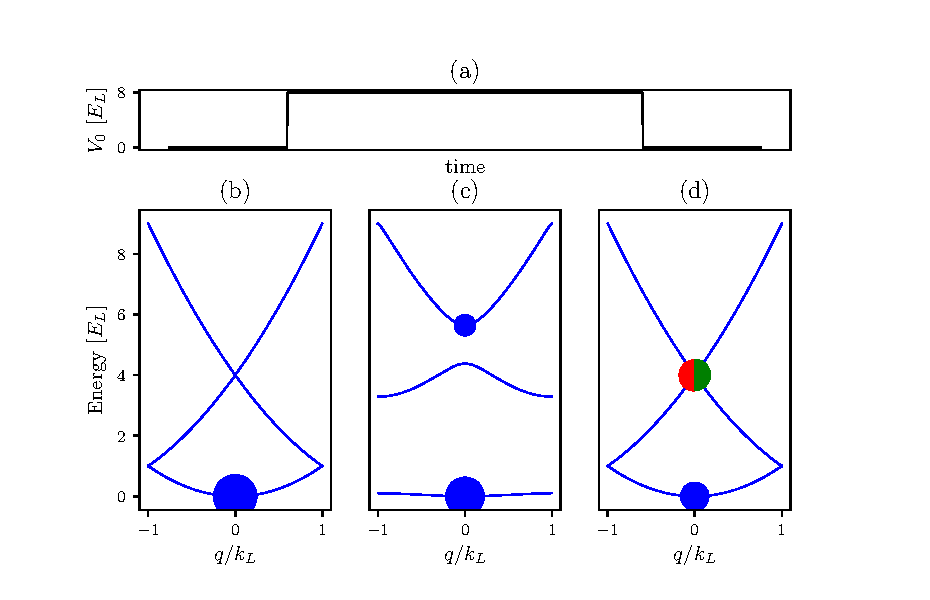
\includegraphics{Chapter4 Figures/figure2.pdf}}
\caption{(a) Dependence of velocity and detuning on position simulated for \K{} at three different imaging times and a probe intensity $\tilde{I}_0=0.8$. (b) Column densities deduced from optical depths obtained from recoil detuning corrected simulation of on-resonant imaging of $^{40}K$ atoms at probe intensity $\tilde{I}_0=0.8$. The input column density $\sigma_0 n=1.6$. $\sigma_0 n^{\rm{(1)}}$ is the high probe intensity corrected column density given by Eq. (\ref{eq2}). $\sigma_0 n^{\rm{(2)}}$ is the column density as expanded to second order in time, Eq. (\ref{eq:OD2}).}
\label{fig:expos}
\end{figure}
\par By considering this equation perturbatively in imaging time we obtain corrections to second order \cite{LJLthesis}

\begin{eqnarray}
&\sigma_0 n^{\rm{(2)}}  =  c_0+c_1t+c_2t^2, \mbox{ where } \\
 &c_0= \sigma_0 n^{\rm{(1)}}, c_1=0, c_2=\frac{( k_{\rm{r}} v_{\rm{r}})^2}{3}\left[\frac{1}{\tilde{I}_f+1}-\frac{1}{\tilde{I}_0+1}+\mathrm{ln}\left(\frac{\tilde{I}_f+1}{\tilde{I}_0+1}\right)\right]
\label{eq:OD2}
\end{eqnarray}
As shown in  Fig. \ref{fig:expos}(b), the perturbative treatment is accurate to times up to the recoil time after which it begins to diverge. To adequately correct for the recoil induced detuning of the atoms, we numerically simulated the imaging process to obtain $\tilde{I}_f$ as a function of imaging time, atomic density, and probe intensity.
%\begin{figure}
%	\includegraphics*{figure2.pdf}
%\caption{Using time dependent $I_f$ values obtained from recoil detuning corrected simulation of on-resonant imaging of $^{40}K$ atoms at probe intensity $I_0=0.8\, I_{\rm{sat}}$, this graph shows the optical depths obtained by each model. The `true' optical depth is $\sigma_0 n=1.6$. $OD_1$ is the high probe intensity corrected optical depth given by Eq. (\ref{eq2}). $OD_2$ is the high probe intensity corrected and expanded to second order in time optical depth, Eq. (\ref{eq:OD2}) \cite{LJLthesis}. The recoil time is the time it takes for the cloud, on average, to become detuned by a linewidth $\Gamma$. Both models start to differ from the true value before a recoil time.  }
%\label{fig:ODcorrections}
%\end{figure}
\par In the following, we describe two versions of this simulation. First, we took a simplistic approach where the spatial distribution of atoms did not change appreciably during the imaging time: $vt\ll I_0/(\hbar \omega_{\rm{L}} \gamma_{\rm{sc}} \rho)$. We verified this approach in known limits and then cross-checked the validity of the static assumption. For realistic input parameters, we found this assumption to be invalid. We then developed a quasi-classical approach and allowed the atoms to move during the imaging time. While the atomic trajectories were wildly different than in the static atom approximation, we found that the predicted $OD$s only differed on the 0.5$\%$ level.


\section{Stationary atom model}
To solve Eqs. (\ref{eq3})-(\ref{eq4}), we divided the cloud into spatial bins.  In this approximation, the number of atoms in each bin was time-independent.  The algorithm used is shown in Alg. (\ref{algorithm1}), in which we took a Gaussian profile for our initial density distribution. We call the optical depth simulated by this algorithm the simulated optical depth $OD^{\rm{sim1}}$.

\begin{algorithm}
\caption{Stationary atom model}
\label{algorithm1}
\begin{algorithmic}
\STATE $I[n=0,t]=I_0$ \COMMENT{$n$ is the bin index, $t$ is the time index, $I$ is in units of $I_{\rm{sat}}$}
\STATE $\delta[n, t=0]=0$ \COMMENT{light initially resonant, $\delta$ in units of $\Gamma/2$}
\STATE $H_f=0$ \COMMENT{Radiant fluence seen by camera after passing through cloud}
\FOR[loop over time steps]{$t=0$ to $t_f$}
 \FOR[loop over bins, N is total bin number]{$n=1$ to $N$}
 \STATE $A=\sigma_0\rho[n] dz$ \COMMENT{$dz$ is the size of spatial step}
 \STATE $B=v_{\rm{r}} dt/(\hbar c \rho[n])$  \COMMENT{$dt$ is the size of the time step}
\STATE $I[n,t]=I[n-1,t] - A I[n-1,t]/(1+\delta[n,t-1]^2+I[n-1,t])$  \COMMENT{Eq. (\ref{eq3})}
\STATE $\delta[n,t]=\delta[n,t-1]+B\left(I[n-1,t]-I[n,t]\right)$  \COMMENT{Eq. (\ref{eq4})}
\ENDFOR
\STATE $H_f =H_f+ I[N,t]dt$ \COMMENT{collecting total fluence seen by the camera}
\ENDFOR
\STATE $OD^{\rm{sim1}}=-\ln{(H_f/I_0t_f)}$
\end{algorithmic}
\end{algorithm}

\par We checked the validity of our simulation in the limits where the problem is analytically solvable. In the limit where the probe intensity is much weaker than the saturation intensity, $\tilde{I}_0\ll 1$, the atoms' velocities are hardly changed, and Eq.(\ref{eq3}) reduces to
\begin{eqnarray}
\frac{d\tilde{I}(z)}{dz}&=-\rho\sigma_0\tilde{I}(z), \mbox{ from which we recover the analytic form }\\
\sigma_0 n^{\rm{(0)}} &= -\ln\tilde{I}_0/\tilde{I}_f. \label{eq6}
\end{eqnarray}
In the limit where the probe intensity is much larger than the saturation intensity, $\tilde{I}_0\gg \tilde{\delta}$, even far detuned atoms will scatter light at their maximum rate. The time dependence of the detuning can thus be neglected, and Eq. (\ref{eq3}) becomes
\begin{eqnarray}
\frac{d\tilde{I}(z)}{dz}&=-\rho\sigma_0, \mbox{ which integrates to }\\
\sigma_0 n &= \tilde{I}_0 - \tilde{I}_f. \label{eq8}
\end{eqnarray}
We recognize the right hand sides of Eq. (\ref{eq6}) and Eq. (\ref{eq8}) as the two terms in Eq. (\ref{eq2}). Thus, as shown in  Fig. \ref{fig:IsatLimits}, $OD^{\rm{sim1}}$  coincides with the optical depth as predicted by Eq. (\ref{eq2}) in both the small and large probe intensity limits.
\begin{figure}
	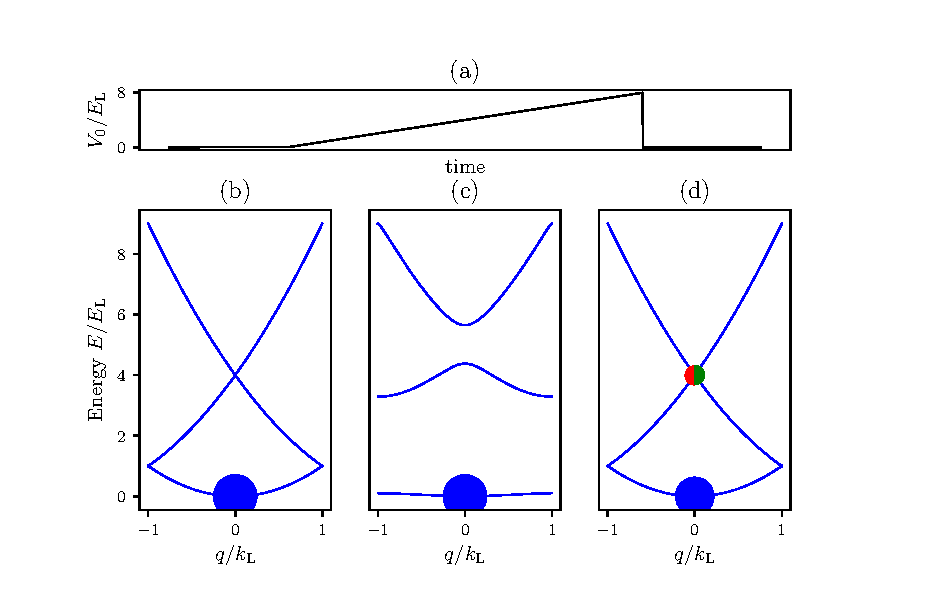
\includegraphics{Chapter4 Figures/figure3.pdf}
\caption{Optical depth as a function of probe intensity as predicted by the simulation (blue symbols) and by Eq. (\ref{eq2}) (green curves), for three different imaging times. As expected, the predictions agree in both the high and low intensity limits, and differ for probe intensities comparable to the saturation intensity and longer imaging times. }
\label{fig:IsatLimits}
\end{figure}
\par We used the results of this simulation to check the self-consistency of the  stationary atom assumption, i.e. the distance traveled by the atoms (as deduced from integrating the acquired recoil velocity over the imaging time) is less than the bin size. As can be seen from Fig. \ref{fig:simTests}(a), not only do the atoms travel more than the bin size, but they travel far beyond the initial extent of the cloud. Moreover, owing to the higher initial scatter rate, the back of the cloud overtakes the front for long imaging times. Thus, the atomic distribution as a function of position changes dramatically during the imaging pulse, and the stationary assumption is invalid.
\begin{figure}
	\subfigure[]{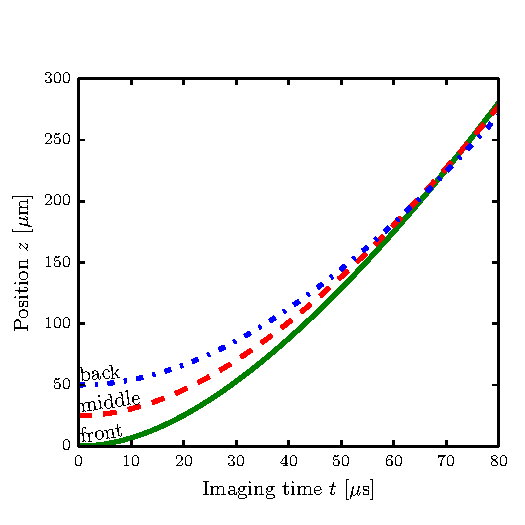
\includegraphics{Chapter4 Figures/figure4.pdf}}
	\subfigure[]{\includegraphics{Chapter4 Figures/figure5.pdf}}
\caption{(a) Position of atoms as a function of imaging time for atoms in the first (solid green), middle (dashed red), and last (dotted blue) bins of the simulated density distribution for an initial cloud 50 \um{} in extent. The probe intensity used in this calculation was $1.2\, I_{\rm{sat}}$, and the column density was $\sigma_0 n=1.6$. (b) The velocity of a single composite atom as a function of probe intensity for various imaging times. Simulation data (dots) and numerical  solutions of Eq. (\ref{eq10}) (lines) are in agreement.}
\label{fig:simTests}
\end{figure}

\section{Traveling atom model}
To account for the changing atomic distribution during the imaging pulse, we numerically simulated the classical kinetics of atoms subject to the recoil driven optical forces. To simulate large ensembles in a reasonable time, we modeled composite atoms, each describing the aggregate behavior of $N_{\rm{ca}}$ atoms. The amended algorithm is shown in Alg. (\ref{algorithm2}).
\begin{algorithm}
\caption{Travelling atom model}
\label{algorithm2}
\begin{algorithmic}
\STATE $z[n]=z_0$, $\delta[n]=0$ \COMMENT{initialize position and detuning for each composite atom, labeled by index $n$}
\STATE $O[i]=n$ \COMMENT{make a list of composite atom indexes, ordered by position}
\STATE $I[n=0,t]=I_0$ \COMMENT{ $t$ is the time index, $I$ is in units of $I_{\rm{sat}}$}
\STATE $H_f=0$ \COMMENT{Radiant fluence seen by camera after passing through cloud}
\FOR[loop over time steps]{$t=0$ to $t_f$}
 \FOR[loop over superatoms]{$i=1$ to $N$}
\STATE $n=O[i]$ \COMMENT{apply probe intensity to composite atoms in order of appearance}
 \STATE $A=\sigma_0 N_{sa} dz$ \COMMENT{dz is length over which atoms were grouped into single composite atom}
 \STATE $B=v_{\rm{r}} dt/(\hbar c  N_{sa})$  \COMMENT{dt is the time step}
\STATE $I[n,t]=I[n-1,t] - A I[n-1,t]/(1+\delta[n]^2+I[n-1,t])$  \COMMENT{Eq. (\ref{eq3})}
\STATE $\delta[n]\mathrel{+}=B\left(I[n-1,t]-I[n,t]\right)$  \COMMENT{Eq. (\ref{eq4}), detuning in units of $\Gamma/2$}
\STATE $z[n]\mathrel{+}=dt\Gamma\delta/2k$ \COMMENT{$k$ is the wavenumber, $\Gamma\delta/2k$ is the velocity at $\delta$ detuning}
\ENDFOR
\STATE $O[i]$=sort($n$, key =$z[n]$) \COMMENT{sort composite atom indexes by current position}
\STATE $H_f H_f+ I[N,t]dt$ \COMMENT{collecting total fluence seen by the camera}
\ENDFOR
\STATE $OD^{\rm{sim2}}=-\ln{(H_f/I_0t_f)}$
\end{algorithmic}
\end{algorithm}
\par To validate our code, we again checked the velocity predicted in this model against known limits. One such limit is that of a single composite atom. In this case, there is no attenuation, and the intensity seen by the composite atom is constant at $\tilde{I}_0$. Only the detuning  evolves in time, and Eqs. (\ref{eq3}) and (\ref{eq4}) give
\begin{equation}
\frac{d\tilde{\delta}(t)}{dt}= \frac{ k_{\rm{r}} v_{\rm{r}}}{2} \frac{\tilde{I}}{1+4\tilde{\delta}^2+\tilde{I}}.
\label{eq10}
\end{equation}
Equation (\ref{eq10}) can be solved numerically, and is in agreement with our simulation, as seen in Fig. \ref{fig:simTests}(b).
%\begin{figure}
%	\includegraphics{figure5.pdf}
%\caption{The velocity of a single superatom as a function of probe intensity for various imaging times. Simulation data (dots) and numerical  solutions of Eq. (\ref{eq10}) (lines) are in good agreement.}
%\label{fig:oneAtomVel}
%\end{figure}
\par We used this model to study the time evolution of the cloud shape during imaging and visualized the phase space evolution of superatoms, shown in Fig. \ref{fig:phaseSpace}. The cloud is strongly distorted during imaging.
\begin{figure}
	\subfigure[]{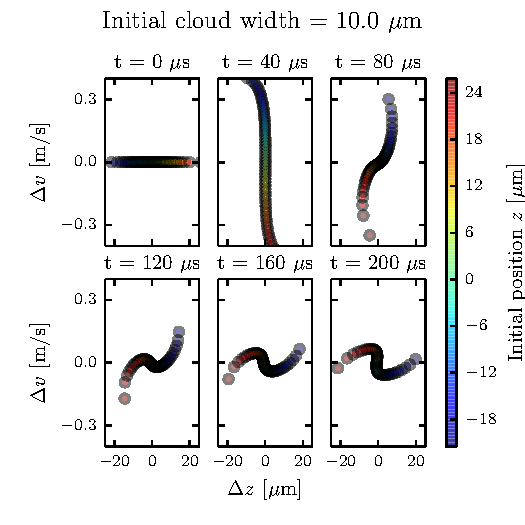
\includegraphics{Chapter4 Figures/figure6a.pdf}}
	\subfigure[]{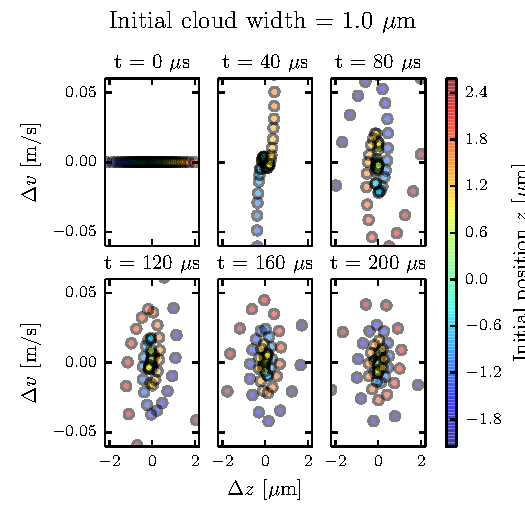
\includegraphics{Chapter4 Figures/figure6b.pdf}}
\caption{Phase space evolution of an atomic cloud exposed to probe light with intensity $\tilde{I}_0=1.2$. We defined $\Delta v=v -\left< v(t) \right>$  and $\Delta z=z-\left< z(t) \right>$, subtracting out the center of mass position and velocity of the cloud. The column density $\sigma_0 n$ is 1.6, and the initial cloud is a Gaussian with a width of 10 $\mu$m in (a) and 1 $\mu$m in (b). The center of mass velocities $\left< v\right>$ are (0,  3.41, 5.26, 6.52, 7.50, 8.32) m/s sequentially, and are the same for both initial cloud widths. }
\label{fig:phaseSpace}
\end{figure}
\par We compared the optical depths predicted by each of the two models, $OD^{\rm{sim1}}$ and $OD^{\rm{sim2}}$. As seen Fig. \ref{fig:compareModelsAndIsat}(a), the predicted optical depths were hardly changed by including the full time evolution:  $\left|OD^{\rm{sim1}}-OD^{\rm{sim2}}\right|/OD^{\rm{sim1}} \le 0.005$. Thus, for the purposes of deducing the atom density from experimental optical depths, the stationary atom model is sufficient. Furthermore, we simulated a range of initial density profiles $\rho(z)$, and found their impact to be negligible \--- the only observable is the integrated atomic density $n=\int\rho(z)\mathrm{d}z$. Still, for interpreting experimental images, we used the data generated by the traveling atom simulation.
\begin{figure}
	\subfigure[]{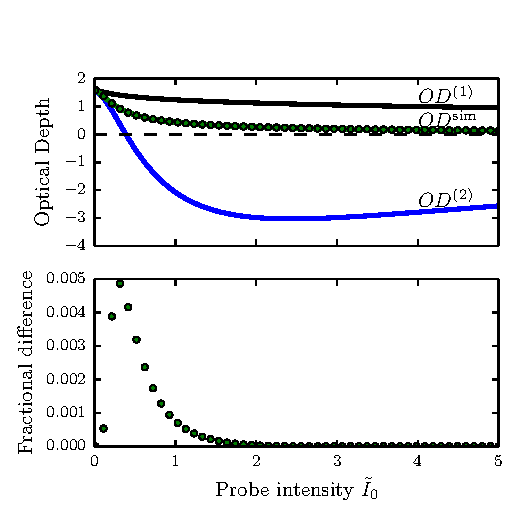
\includegraphics{Chapter4 Figures/figure7.pdf}}
	\subfigure[]{\includegraphics{Chapter4 Figures/figure8.pdf}}
\caption{(a) Top. Optical depth as a function of probe intensity for an imaging time $t=100$ \us. $OD^{\rm{(1)}}$ and $OD^{\rm{(2)}}$ are optical depths predicted from a given column density by Eq. (\ref{eq2}) and (\ref{eq:OD2}) respectively.  The two versions of simulated optical depth, $OD^{\rm{sim1}}$ (green curve) and $OD^{\rm{sim2}}$ (green dots) are plotted. Bottom. The fractional difference between two versions of the simulated $OD$, $\left|OD^{\rm{sim1}}-OD^{\rm{sim2}}\right|/OD^{\rm{sim1}}$. (b) The optical depth as a function of probe intensity for three imaging times: $t=40$ \us{} (cyan),  $t=75$ \us{} (magenta),  $t=100$ \us{} (red). The dots represent experimental data and the lines represent the best fit of simulated data. The optimal fit parameters pictured are a $\sigma_0 n$ of 1.627(5) and saturation intensity of 29(7) counts/\us{}.  }
\label{fig:compareModelsAndIsat}
\end{figure}

\section{SNR optimization}
This simulation allowed us to interpret experimental data. For a given imaging time, we created a look-up table of predicted optical depth as a function of probe intensity and atomic column density. We then found the observed optical depth on this table, with the given probe intensity, and inferred the atomic density. The uncertainty in the measured intensities can be propagated through this procedure, and we established optimal imaging parameters to maximize the SNR of this detection scheme.
\par The only source of measurement uncertainty we considered was the Poisson noise on the detected arriving photons (i.e., photoelectrons) with standard deviation proportional to $q_{\rm{e}}\sqrt{N_p}$, where $q_{\rm{e}}$ is the quantum efficiency of the camera and $N_p$ is the photon number. We then propagated this uncertainty through our correction scheme to obtain the uncertainty in our deduced value of $\sigma_0 n$. We define the SNR as $\sigma_0 n/\delta_{\sigma_0 n}$, where $ \delta_{\sigma_0 n}$ is the propagated measurement uncertainty.
\par As seen in Fig. \ref{fig:SNR}(a), after about 40 \us{} extending the imaging time no longer yields appreciable improvement in SNR. Imaging for 40 \us{} as opposed to 10 \us{} where the uncorrected model is appropriate, improves the SNR by a factor of  1.5. We performed the experiments described in the second section at 40 \us{} imaging time. Figure \ref{fig:SNR}(b) shows that the optimal probe intensity varies with the atomic column density. For low atom numbers, $\sigma_0 n\approx0.1$, a probe intensity of $\tilde{I}_0\approx0.6$ is best. However, in our experiment the probe intensity had a Gaussian profile and was not uniform over the whole image.  The typical probe intensities used in our experiments varied over the $2\tilde{I}_0=0.1-0.7$  range.
\begin{figure}
	\subfigure[]{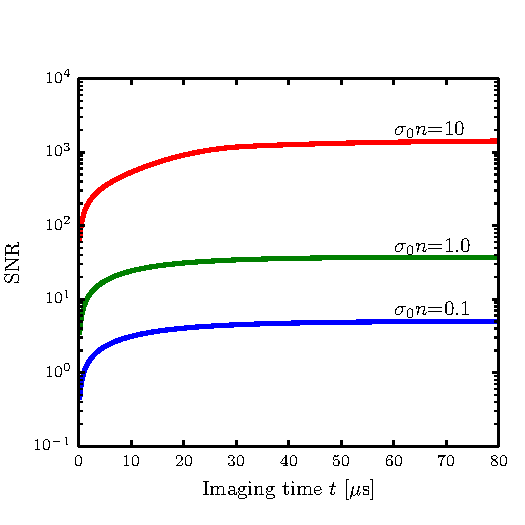
\includegraphics{Chapter4 Figures/figure9a.pdf}}
	\subfigure[]{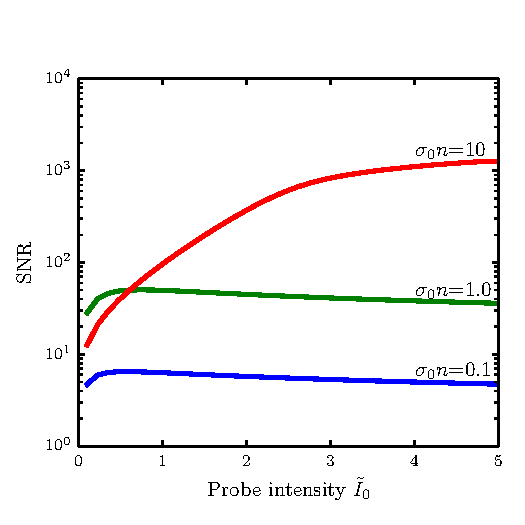
\includegraphics{Chapter4 Figures/figure9b.pdf}}
\caption{SNR for three different column densities after correcting for recoil induced detuning. (a) SNR as a function of imaging time for a probe intensity of $\tilde{I}_0=5.0$ and (b) SNR as a function of probe intensity for an imaging time of 50 \us{}.}
\label{fig:SNR}
\end{figure}

\section{Calibration of saturation intensity}
Our absorption images were taking using a charge-coupled device (CCD) camera.  Each camera pixel  converted the photons it was exposed to, with some efficiency, into photoelectrons, and digitally returned an integer, called `counts', that was proportional to the radiant fluence.  However, the proportionality constant depends on many factors, such as the quantum efficiency of the camera, the electronic gain during the readout process, losses in the imaging system and the polarization of the probe light.
\par We determined this proportionality constant through direct measurement. In the limit where the system is adequately described by $\sigma_0 n=-\ln(\tilde{I}_f/\tilde{I}_0)$, only the ratio of the initial and final intensities matter, and this proportionality constant is irrelevant. In all other regimes, however, the ratio of the initial and final intensities to the saturation intensity also comes into play, making the proportionality constant significant. One way to approach this calibration is to determine the saturation intensity in units of `counts' per unit time.
\par To calibrate the saturation intensity in camera counts per unit time, we took absorption images of \K{} clouds at three different imaging times (40 \us{}, 100 \us{}, and 200 \us{}) with varying probe intensities. In a small region at the center of the cloud the atomic density was approximately uniform, and we averaged the initial and final intensities of each pixel in that region. Thus, for each image we obtained $\tilde{I}_0$ and $\tilde{I}_f$, in counts per microsecond. We then simultaneously fit our simulated optical depth  $OD^{\rm{sim}}$ to this full data set, with the atomic density $\sigma_0 n$ and  $I_{\rm{sat}}$ in counts per microsecond as free parameters. As seen in Fig. \ref{fig:compareModelsAndIsat}(b), the model produced a good fit to the experimental data, and provided a calibration of the saturation intensity for our experiment.
%\begin{figure}
%	\includegraphics{figure8.pdf}
%\caption{The optical depth as a function of probe intensity for three imaging times: $t=40$\us{} (blue),  $t=75$\us{} (green),  $t=100$\us{} (red). The dots represent experimental data and the lines represent the best fit of simulated data. The optimal fit parameters pictured are a $\sigma_0 n$ of 1.62 and saturation intensity of 29 counts/\us{}. }
%\label{fig:isatCalib}
%\end{figure}
